\textbf{Group exercise}
	
	We have a continuous feature and outcome $(Y, X) \in \R^2$ and denote $f(x)$ as the true prediction function. 
	The following sketches out the data and $f(x)$.
	\begin{figure}[H]
		\centering
		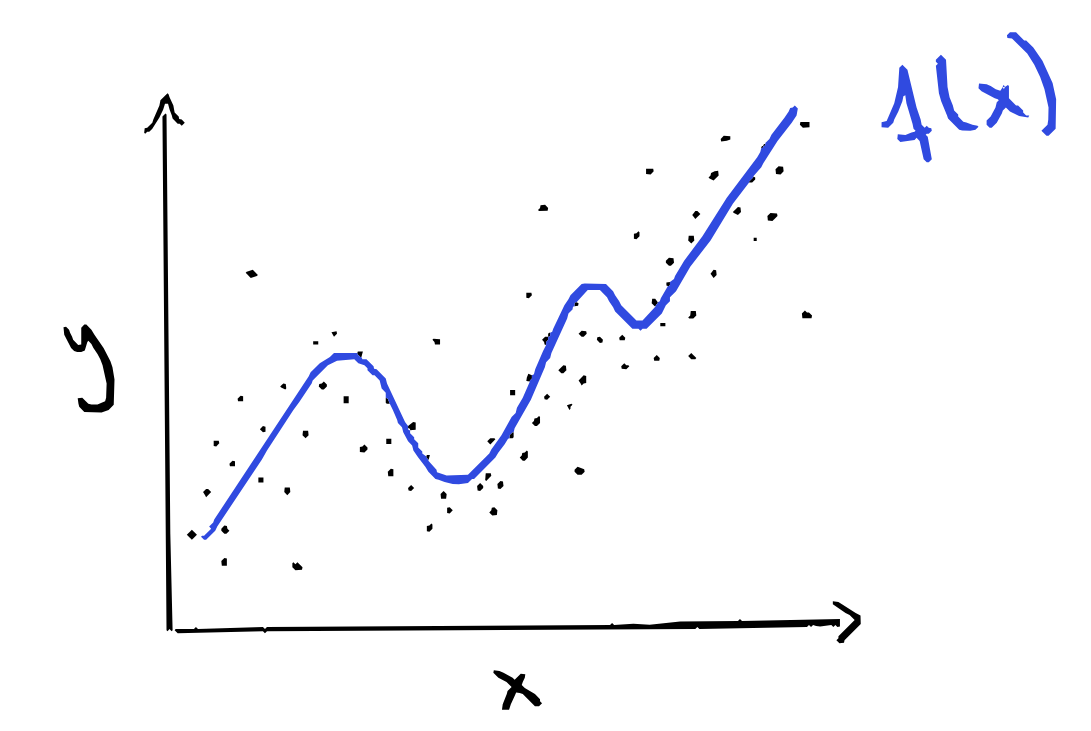
\includegraphics[width=.3\textwidth]{ex_tex/complexity_example_plot.png}
	\end{figure}

	\begin{enumerate}
		\item Sketch out in the above plot how the following prediction functions $\fh(x)$ would approximate the true $f(x)$.
		\begin{itemize}
			\item[A] Linear regression model: $\fh(x) = \thetah_0 + \thetah_1 x$
			\item[B] Polynomial regression model of order $20$: $\fh(x) = \thetah_0 + \thetah_1 x + \thetah_2 x^2 + ... + \thetah_{20} x^{20}$
			\item[C] Regression tree of depth $2$: $\fh(x) = \sum\limits_{m=1}^4 \hat c_m \mathds{1}_{\{x \in \mathcal{R}_m\}}$ (assume full binary structure)
			
			\hspace{3cm}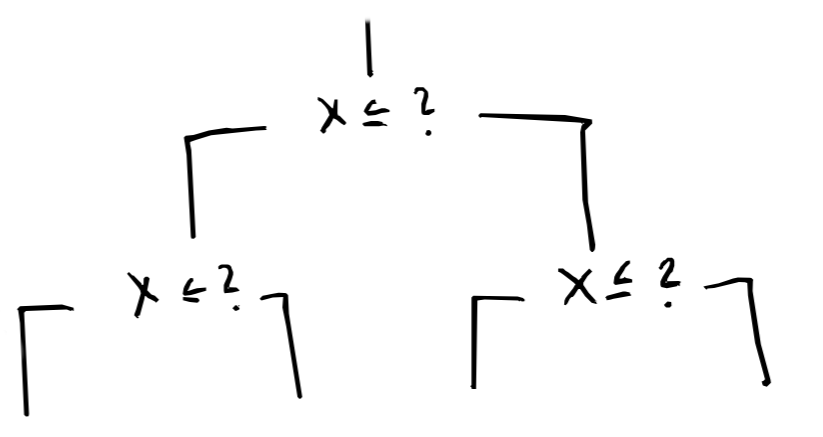
\includegraphics[width = .3\textwidth, ]{ex_tex/complexity_example_plot2.png}
			\item[D] Regression tree of depth $10$: $\fh(x) = \sum\limits_{m=1}^{2^{10}} \hat c_m \mathds{1}_{\{x \in \mathcal{R}_m\}}$ (assume full binary structure)
			\item[E] Tuned generalized linear model (with splines, penalized with optimal smoothness parameter chosen via cross-validation): $\fh(x) = \thetah_0 + \fh_1(x)$
		\end{itemize}
		\item How would you measure complexity of the models? Your measure should be model-agnostic, i.e., applicable across all model classes (not specific to linear models or trees). 
		Order the above models A - E by your specified complexity measure. 
		
		\textit{Hint}: Think about the model parameters or effect approximations, etc.

	\end{enumerate}






